\chapter{Object-oriëntatie}
We hebben het al gehad over object-georiënteerd programmeren
in Java, maar wat zijn precies de ideeën hierachter?
Hoe kunnen we objecten inzetten om separation of concerns,
loose coupling en high cohesion te bereiken?

Hiervoor is het zinvol om stil te staan bij de algemene eigenschappen 
zijn object-oriëntatie. We sluiten hierbij aan 
bij het objectmodel uit het boek 
Object-Oriented Analysis and Design with Applications 
van object- en UML-pionier Grady Booch en anderen. 
Hierin staan een aantal belangrijke en minder belangrijke 
elementen die in object-georiënteerde projecten voorkomen. 
Deze elementen kan je ook tegenkomen bij andere stijlen van programmeren,
maar wij staan vooral stil bij hoe deze elementen gebruikt kunnen worden 
in een object-georiënteerde taal. Hoe kunnen we deze elementen benutten 
om tot een sterk ontwerp te komen?

\section{Het objectmodel van Booch}
Het objectmodel van Booch onderscheidt vier belangrijke elementen 
die een rol spelen bij het object-georiënteerd modelleren:
\footnote{
    In de praktijk wordt ook wel eens verwezen naar de \texit{4 Pillars of Object Orientation}: 
    abstraction, encapsulation, polymorphism en inheritance. 
    Deze zijn in het objectmodel van Booch inbegrepen.
}
\begin{enumerate}
    \item Abstraction
    \item Encapsulation 
    \item Modularity 
    \item Hierarchy
\end{enumerate}

Deze onderdelen noemen Booch et al. belangrijk omdat je 
zonder deze elementen geen object-georiënteerde taal (OO-taal) kan hebben.
Daarnaast beschrijven zij drie minder belangrijke elementen die je 
bij veel OO-talen tegen kunt komen: typing, persistence en concurrency.

Dit betekent natuurlijk niet dat je deze zaken buiten OO-talen niet tegen zal komen! 

\subsection{Abstraction}
In een object-georiënteerde taal zijn objecten de abstracties 
waarmee we werken. Het is niet de bedoeling van een abstractie 
om de wereld precies na te bootsen.
We willen concepten modelleren voor zover deze van belang zijn 
voor het domein van de applicatie en het betreffende programmaonderdeel.
In een object zijn toestand (fields) en gedrag (methods) samengebracht
om een bepaalde rol binnen een systeem te vervullen.

\blockquote{
    An abstraction denotes the essential characteristics 
    of an object that distinguish it from all other kinds 
    of objects and thus provide crisply defined conceptual
    boundaries, relative to the perspective of the viewer.
}{\cite{Booch2007}, p. 44.}

Een manier om te kijken naar abstractie is door 
het object te beschouwen van de buitenkant. 
We zien manieren om met het object te interacteren,
maar we kunnen niet naar binnen kijken of invloed 
uitoefenen op de interne structuur of hoe het object
precies omgaat met die interactie.
\cite{Abelson1996} noemen dit een \textit{abstraction barrier}
 in hoofdstuk 2 van het invloedrijke boek 
Structure en Interpretation of Computer Programs.
Als gebruiker van een object kunnen we alleen maar 
zien tot de "grens" van een abstractie en niet daar voorbij.
We kunnen alleen interacteren met het protocol (de API) van 
het object: diens publieke method signatures.
In Java en veel andere talen kan je dit protocol afdwingen
met behulp van \textit{interfaces}. De interne implementatie 
van een object is dus verborgen. 
Dit noemt men ook wel \textit{implementation hiding}.

Liskov en Zilles beschreven in hun zoektocht naar 
programmeren met abstracties een dergelijke grens:
\blockquote{
    When a programmer makes use of an abstract data object,
    he is concerned only with the behavior which 
    that object exhibits but not with any details of how that 
    behavior is achieved by means of an implementation.
    The behavior of an object is captured by the set of 
    characterizing operations.
    \newline\newline
    (...)
    \newline\newline
    Implementation information (...)
    is only needed when defining how the characterizing 
    operations are to be implemented.
    The user of the object is not required to know 
    or supply this information.
}{\cite{Liskov1974}, p. 51.}

Het voordeel van het werken met abstracties is dus 
dat we ons niet bezig hoeven te houden met de precieze
interne werking van een object, maar als buitenstaanders 
ons slechts hoeven te concentreren op de aangebode publieke 
methodes. 

Bij een digitaal kaart- of bordspel zou je een abstractie kunnen 
aanmaken voor het spelpotje zelf, zodat de gehele speltoestand 
opgeslagen kan worden. Acties die door de speler(s) op het spel 
kunnen worden uitgevoerd kunnen dan opgenomen worden als methodes
op het spelpotje. De verschillende onderdelen en concepten binnen 
het spel zou je kunnen opnemen als aparte objecten met hun eigen 
velden, methodes en regels. Concepten die in het spel voorkomen 
kunnen gemodelleerd worden als objecten die op hun beurt weer 
van slimme, beschrijvende methodes kunnen worden voorzien. 
Denk bijvoorbeeld aan een object 
waar bepaalde spelregels in zijn opgenomen, aan alles wat je binnen 
een spel met een kaart kan doen of bijvoorbeeld het onderscheid tussen 
een pakje kaarten en een hand met kaarten. Elke abstractie heeft zijn 
eigen toestand en gedrag. Met een beetje goede naamgeving leest 
de code dan ook als een samenvatting van spelacties!

Met abstraction kunnen we cohesion verhogen door zaken 
bij elkaar te stoppen die bij elkaar 
horen en koppeling verminderen door afhankelijk te zijn van de 
API van een object in plaats van diens interne implementatiedetails.

\subsection{Encapsulation}
Encapsulation and abstraction zijn twee kanten van dezelfde 
medaille. Abstraction is een perpectief van buitenaf: 
wat voor interactiemogelijkheden biedt een object 
en hoe gedraagt dit object zich?
\textit{Encapsulation} (of: inkapseling) 
richt zich meer op de binnenkant:
hoe wordt het interne gedrag afgeschermd van de 
buitenwereld? Object-georiënteerde code benut 
encapsulation op koppeling te reduceren.

\blockquote{Encapsulation is the process 
of compartmentalizing the elements of an 
abstraction that constitute its structure and 
behavior; encapsulation serves to separate the
contractual interface of an abstraction and its 
implementation.}{\cite{Booch2007}, p. 52.}

\textit{Information hiding} speelt hierbij een belangrijke 
rol: we willen niet hebben dat elk object bij elkaars 
interne datastructuren kan komen. In plaats daarvan 
willen we controle uitoefenen over de afhankelijkheden.
Door informatie te verbergen kan je namelijk het aantal 
en de ingrijpendheid van afhankelijkheden tussen 
klassen verminderen. Hiervoor gebruiken we in Java
de access modifier \textit{private}.
Het moderne begrip van encapsulation is gebaseerd op 
Parnas-modules, genoemd naar David Parnas.
Hij beschreef afhankelijkheden als \emph{connections}
en vond dat connecties niet teveel informatie mochten prijsgeven.
\blockquote{
    The connections between modules are the assumptions
    which the modules make about each other.
    \newline\newline
    (...)
    \newline\newline
    We ask, ``What changes can be made to one module
    without involving change to other modules?'' 
    We may make only those changes which do not violate
    the module being changed. In other words,
    a single module may be changed only while the `connections'
    still `fit'. Here, too, we have a strong argument for
    for making the connections contain as little information as possible.
}{\cite{Parnas1971}, pp. 339-340}

Encapsulation, in het bijzonder information hiding,
kan dus helpen om het aantal afhankelijkheden te reduceren
en dus koppeling te verlagen. 

We hebben als het ware een \textit{capsule}
waarbinnen de kern van heb object ligt besloten en kunnen alleen met die 
capsule praten via de publieke methoden. Om die reden willen we voorzichtig
zijn met het \texttt{public} maken van fields of het standaard toevoegen van 
getters en setters. Dit vergroot de kans dat buitenstaande objecten gekoppeld 
raken aan de interne structuur van een object. Door alleen te koppelen tegen 
de publieke methodes van een object, is het makkelijker om de interne toestand 
van het object te wijzigen.

\subsubsection{Tell, Don't Ask}
Een algemene vuistregel om het gebruik van getters en setters te verminderen,
is \textit{Tell, don't ask}. Hiermee wordt bedoeld dat je liever tegen een object 
wil zeggen wat het moet doen, in plaats van dat je alle informatie eruit trekt
er wat mee doet en het vervolgens weer terug in het object stopt. 
Dit wordt wat versimpeld weergegeven in Voorbeeld~\ref{code:tell-dont-ask}.
In de echte wereld zou je natuurlijk liever de geboortedatum van de persoon 
opslaan en heb je dit probleem niet.

\begin{listing}[H]
\begin{minted}[linenos]{java}
String name = "Alex";
Integer age = 31;
Person person = new Person(name, age);

// Don't make a "dumb" object...
Integer afterBirthday = person.getAge() + 1;
person.setAge(afterBirthday);

// Rather, let the object do the work!
person.celebrateBirthday();
\end{minted}
\caption{\textit{Tell, don't ask} houdt in dat je het object het werk laat doen.
Bijkomstig voordeel is dat de bedoeling van de actie duidelijk wordt.}
\label{code:tell-dont-ask}
\end{listing}

Op deze manier reduceer je niet alleen de koppeling, 
je maakt een object meer samenhangend omdat de logica 
die hoort bij wat het betreffende object vertegenwoordigt
onderdeel is van het object. Het hoort bij diens verantwoordelijkheid.
Je kan een boel versimpelen door minder met getters en setters te werken!

\subsubsection{Law of Demeter}
De \textit{Law of Demeter} of \textit{the principle of least knowledge} 
is een extra richtlijn om encapsulation in te richten en koppeling te reduceren
(\cite{Lieberherr1989}). In de praktijk wordt dit vaak als volgt samengevat:

\begin{itemize}
    \item Objecten mogen slechts kennis hebben van andere objecten als ze nauw eraan verwant zijn
    \item Objecten mogen alleen praten met vrienden, niet met vreemden
    \item Objecten mogen alleen praten met directe vrienden, niet met vrienden van vrienden
\end{itemize}

Probeer objecten dus alleen met elkaar te laten praten als ze 
structureel met elkaar samenhangen of als ze een duidelijke dienst afnemen.
Als het gaat om een dienst, praat dan met het object dat de dienst verleent 
en ga niet met de objecten praten die dat dienstverlendende object gebruikt om
de dienst te vervullen. 
In andere woorden: koppel niet tegen de interne representatie van een object!

Helaas werken veel object-georiënteerde projecten niet volgens dit principe en 
is de code met getters in elkaar geknoopt. 
Zo koppel je buitenstaande objecten niet alleen op de 
interne toestand van één object, maar op de interne toestanden van 
de objecten die daarin liggen besloten. Zie Voorbeeld~\ref{code:train-wreck}.

\begin{listing}[H]
\begin{minted}[linenos]{java}
// A client class, for example: Main.java
Result result;
Integer player1Score = game.getCurrentRound().getPlayer1().getScore();
Integer player2Score = game.getCurrentRound().getPlayer2().getScore();

if (player1Score > player2Score) {
    result = Result.PLAYER_ONE_WON;
} else if (player2Score > player1Score) {
    result = Result.PLAYER_TWO_WON;
} else {
    result = Result.DRAW;
}
\end{minted}
\caption{Dit is een \textit{train wreck} en een overtreding van \textit{the Law of Demeter}.
We moeten namelijk de innerlijke structuur van \texttt{Game}, \texttt{Round} en \texttt{Player} weten.
Dit introduceert meer coupling dan noodzakelijk!}
\label{code:train-wreck}
\end{listing}

Dit is wat men ook wel een 
\textit{train wreck} noemt, omdat de method calls achterelkaar een soort 
treintje met wagonnetjes vormen (\texttt{game.getCurrentRound().getPlayer1().getScore()}).

Om dit tegen te gaan, kan je \textit{Tell, don't ask} toepassen 
om encapsulation te bereiken en te koppelen tegen de abstractie: 
vertel de objecten wat ze moeten doen, in plaats van alle data eruit te trekken.
De externe coupling is dan kleiner, omdat we de interne cohesie benutten.

\begin{listing}[H]
\begin{minted}[linenos]{java}
// A client class, for example: Main.java
Result result = game.evaluateCurrentRound();

// Inside Game.java:
public Result evaluateCurrentRound() {
    // getCurrentRound is a private method
    Round round = this.getCurrentRound();
    return round.evaluate();
}

// Inside Round.java:
public Result evaluate() {
    if (player1.scoredHigherThan(player2)) {
        return Result.PLAYER_ONE_WON;
    } else if (player2.scoredHigherThan(player1)) {
        return Result.PLAYER_TWO_WON;
    } else {
        return Result.DRAW;
    }
}

// Inside Player.java:
public Boolean scoredHigherThan(Player other) {
    // Note: instances can access private fields of other instances of the same class
    return this.score > other.score;
}

\end{minted}
\caption{We reduceren de coupling van buitenaf door meer gebruik te maken van de 
kracht van samenhangende, doelgerichte objecten.}
\label{code:train-wreck-solution}
\end{listing}

In sommige gevallen ontkom je niet aan het gebruik maken van getters.
Dit is vaak het geval bij \textit{serializatie} van objecten naar een ander formaat.
Denk bijvoorbeeld aan het omzetten van een object naar een JSON-representatie 
of naar een SQL-query. Omdat dit gewoonlijk aan de randen van je applicatie gebeurt,
wordt hiervoor vaak \textit{data transfer objects (DTOs)} voor ingezet.

\subsection{Modularity}
Volgens \cite{Booch2007} zijn object-georiënteerde projecten
onderhoudbaar ingericht dankzij \textit{modularity}.

\blockquote{
    Modularity is the property of a system
    that has been decomposed into a set
    of cohesive and loosely coupled modules.    
}{\cite{Booch2007}, p. 56.}

Klassen, packages en interfaces zijn de belangrijkste modules binnen 
een object-georiënteerd project. Zie hierover uitgebreid het hoofdstuk 
over object-georiënteerd programmeren in Java.

In Java brengen we toestand (fields) en gedrag (methods) samen 
in klassen en kunnen we klassen groeperen middels packages.
Interfaces kunnen helpen om, dankzij polymorfisme, abstractie en 
implementatie van elkaar te scheiden en zodoende programmaonderdelen 
van elkaar los te koppelen. Met enums kunnen we het aantal mogelijkheden 
beperken. Generics helpen ons om (geparameterizeerde) containertypen te 
maken waarvan de interne types kunnen variëren dankzij type arguments.
Deze modules helpen ons een \textit{separation of concerns} te bereiken.

\subsection{Hierarchy}
Hiërarchie is een ander element van het werken met objecten om een 
project onderhoudbaar te houden.

\blockquote{
    Hierarchy is a ranking or ordering of abstractions.
}{\cite{Booch2007}, p. 58.}

Met de juiste naamgeving en een intelligente package structuur 
kunnen we een onderhoudbare \textit{softwarearchitectuur} opzetten, waarin 
packages een rol van betekenis vervullen. We brengen daarmee een 
hiërarchie aan in ons softwareproject: een bewuste rangschikking van waar welke 
packages te vinden zijn.

Binnen het domein kunnen we ook een objecthiërarchie waarnemen:
vaak hebben we één object die verantwoordelijk is voor het uitvoeren van 
de domeinacties. Meestal bestaat dit object weer uit allemaal andere objecten
die elk hun eigen velden, methodes en regels bevatten. Op die manier blijft 
niet alleen de code overzichtelijk en kan je onderdelen uitwisselen, de code 
kan soms lezen als een natuurgetrouwe weergave van acties --- met hier en daar 
wat Java-syntax ertussen.

Laten we wat dieper ingaan op deze objecthiërarchie. 
Objecten en klassen staan namelijk niet op zichzelf.
Ze vertonen allerlei relaties tot elkaar. In de meest algemene 
zin kan een object kan een ander object gebruiken (\textit{afhankelijkheid}).
Dit algemene gebruik kan verder worden gespecifieerd. Een object kan 
bijvoorbeeld zijn opgebouwd uit andere objecten (\textit{associatie, aggregatie, compositie}).
Ook kan een klasse een interface implementeren (\textit{realisatie}) of
van een andere klasse fields en methods overerven (\textit{overerving}).
Laten we deze dependency types nader onderzoeken aan de hand 
van de Unified Modeling Language (UML), zoals genoemd in \cite{Booch1999}.

\subsubsection{Afhankelijkheid (`gebruikt')}
Een \textit{afhankelijkheid} (\textit{dependency}) geeft aan dat 
de werking van een bepaalde module op de een of andere manier afhangt
van een andere module. We zeggen ook wel dat de ene module de andere 
module gebruikt.

\blockquote{
    A dependency is a using relationship that states
    that a change in specification of one thing (...)
    may affect another thing that uses it, 
    but not necessarily the reverse.    
}{\cite{Booch1999}, p. 63.}

Zie bijvoorbeeld de withdrawChips-methode in de ChipsService 
van het chips-component het casinoproject (Voorbeeld~\ref{code:withdraw-chips}). 
We halen een Chips-object op uit de ChipsRepository 
via \texttt{this.findChipsByUsername(username)}).
Onze ChipsService \textit{gebruikt} dus de Chips-klasse!

\begin{listing}[H]
\begin{minted}[linenos]{java}
public Balance withdrawChips(String username, Long amount) {
    Chips chips = this.findChipsByUsername(username);

    chips.withdraw(amount);
    this.chipsRepository.save(chips);

    return this.showBalanceFor(chips);
}
\end{minted}
\caption{De \texttt{withdrawChips}-methode uit de ChipsService.}
\label{code:withdraw-chips}
\end{listing}

In een UML-klassediagram zouden we dat (versimpeld) weergeven 
als in Figuur~\ref{fig:uml-dependency}.

\begin{figure}[H]
    \centering
    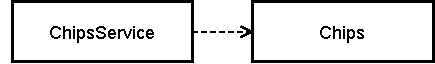
\includegraphics[width=.6\linewidth]{uml-dependency}
    \caption{ChipsService gebruikt de Chips-klasse}
    \label{fig:uml-dependency}
\end{figure}

Je modelleert een relatie als een algemene afhankelijkheid 
als je niet verder kunt of hoeft te specificeren om wat 
voor een soort afhankelijkheid het gaat. Het is vaak wel 
aan te raden om wat dieper te kijken naar het soort relatie
dat de afhankelijkheid vormt.

\subsubsection{Associatie (`zit vast aan')}
Een \textit{associatie} is een algemene manier om te beschrijven dat een 
bepaald object structureel verbonden is met een ander object.
Dit betekent dat het ene object, of een referentie daaraan, 
op de een of andere manier opgenomen is in het andere object.
Dit zie je meestal terug als een \textit{field declaration}
in de klasse. In UML neem je de association echter niet 
op in de klasse, maar wordt deze vertegenwoordigt door een 
lijn of een pijl. Bij een associatie geef je de rolnaam en de 
multipliciteit aan. Een rolnaam komt doorgaans overeen met 
de \textit{field name} en de multipliciteit is een bereik 
van 0 tot 1, 0 tot meer of 1 tot meer. We geven een 
multipliciteitswaarde van "tot meer" aan als het veld is 
gedefinieerd als een collectie.
Een multipliciteitswaarde kan 0 
zijn als de structurele verbinding optioneel is. Dit is het 
geval wanneer het veld conceptueel \texttt{null} mag zijn. 
Naast deze bereiken kan het voorkomen dat een associatie 
exact 1 keer is gevuld.

Een associatie geef je in UML aan met een reguliere pijl om 
de richting aan te geven. Werkt de associatie echter beide kanten op,
dan zijn de pijlhoofden weggelaten. Het betreft dan een streep.
Let ook hier op de rolnamen en multipliciteiten. Deze moeten worden 
opgenomen aan beide kanten!

\blockquote{
    An association is a structural relationship that specifies that objects
    of one thing are connected to objects of another.
}{\cite{Booch1999}, p. 66.}

In Figuur~\ref{fig:uml-association} zien we een voorbeeld van een associatie.
Dit voorbeeld betreft de studentenadministratie van een school.
We kunnen zien dat er een Registration-klasse is waarin een
veld is gedeclareerd van het type \texttt{PaymentMethod} met de naam \texttt{payment}.
Er wordt gebruik gemaakt van een enumeration (enum), 
omdat er in dit voorbeeld maar een beperkt aantal betalingswijzen mogelijk zijn,
 denk aan een maandelijkse overschrijving, of een jaarlijkse automatische incasso.

\begin{figure}[H]
    \centering
    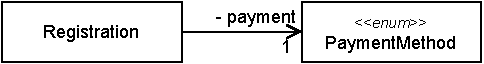
\includegraphics[width=.6\linewidth]{uml-association}
    \caption{Een registratie bevat een betalingswijze.}
    \label{fig:uml-association}
\end{figure}

We gebruiken een associatie om een algemene structurele verbinding aan te 
geven tussen twee klassen.

\subsubsection{Aggregatie (`heeft een')}
Wil je van een associatie specifiek aangeven dat het om een 
deel/geheel-relatie gaat, dan kan je de \textit{aggregatie} gebruiken.

\blockquote{
    Sometimes, you will want to model a "whole/part" relationship,
    in which one class represents a larger thing (the "whole"),
    which consists of smaller things (the "parts"). This kind of
    relationship is called aggregation, which represents a "has-a"
    relationship, meaning that an object of the whole has objects
    of the part.
}{\cite{Booch1999}, p. 67.}

Figuur~\ref{fig:uml-aggregation} laat een voorbeeld van een aggregatie zien.
Een school heeft inschrijvingen.

\begin{figure}[H]
    \centering
    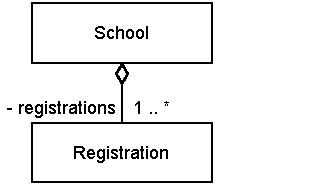
\includegraphics[height=.3\linewidth]{uml-aggregation}
    \caption{Inschrijvingen zijn onderdeel van een school, maar een school kan bestaan zonder inschrijvingen,
    bijvoorbeeld wanneer deze nog in oprichting is.}
    \label{fig:uml-aggregation}
\end{figure}

\subsubsection{Compositie (`is alleen onderdeel van')}
Wil je aangeven van de aggregatie dat het alleen onderdeel
mag zijn van deze klasse en dus niet van andere klassen,
dan geef je dat aan met een \textit{compositie}.
Dat houdt ook in dat de levensduur van de objectinstantie (deel)
gekoppeld is aan de levensduur van de objectinstantie (geheel)
waar het onderdeel van is. Over het algemeen zal een UML compositie 
dus minder snel vervangbaar zijn opgezet dan een UML aggregatie.

\blockquote{
    Composition is a form of aggregation, 
    with strong ownership and coincident lifetime
    as part of the whole. Parts with non-fixed multiplicity 
    may be created after the composite itself,
    but once created they live and die with it. 
    Such parts can also be explicitly removed before the 
    death of a composite.
    \newline\newline
    This means that, in a composite aggregation, 
    an object may be part of only one composite at a time.
    (...) This is in contrast to simple aggregation, 
    in which a part may be shared by several wholes. 
    (...) In addition, in composite aggregation (...) 
    the composite must manage the creation and destruction of its parts.
}{\cite{Booch1999}, p. 147.}

In Figuur~\ref{fig:uml-composition} is een voorbeeld van compositie te zien 
in ons voorbeeld van de schooladministratie. Volgens dit model kan een student 
niet op zichzelf bestaan, maar is altijd onderdeel van een inschrijving. 
In dit model zal het studentnummer dus gekoppeld zijn aan de inschrijving, terwijl 
in de studentklasse misschien persoonlijke informatie is opgenomen, 
zoals geboortedatum, naam, adres en woonplaats. In de praktijk zal dit op een andere
wijze gemodelleerd kunnen worden.

\begin{figure}[H]
    \centering
    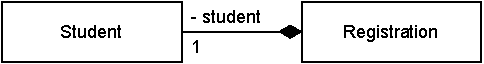
\includegraphics[width=.6\linewidth]{uml-composition}
    \caption{Een inschrijving moet altijd een student betreffen. 
    Een student kan binnen de school niet bestaan zonder inschrijving.}
    \label{fig:uml-composition}
\end{figure}

Volgens de definitie in UML is compositie dus een zeer strikte vorm 
van aggregatie. Deze definitie wordt in de praktijk echter niet zo 
strikt gehanteerd. Dit heeft te maken met het feit dat compositie 
ook een begrip is in bijvoorbeeld niet-object-georiënteerde 
talen, maar ook in wiskunde en de kunsten. In algemene zin betekent
compositie immers `samenstelling'. Dit komt meer overeen met waar 
UML de term `aggregatie' voor gebruikt.

In Figuur~\ref{fig:uml-association-aggregation-composition} zien we 
association, aggregatie en compositie in één model. Het laat zien dat je 
met een relatief eenvoudig diagram complexe ideeën kunt delen.

\begin{figure}[H]
    \centering
    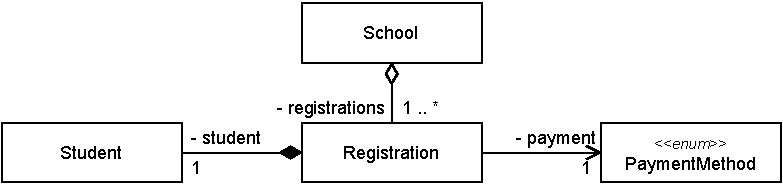
\includegraphics[width=.9\linewidth]{uml-association-aggregation-composition}
    \caption{Association, aggregatie en compositie in één model.}
    \label{fig:uml-association-aggregation-composition}
\end{figure}

\subsubsection{Overerving (`is een soort')}
Overerving (\textit{implementation inheritance}) 
geeft aan dat de subklasse (\textit{child}) een 
specifieke soort is van de superklasse (\textit{parent}) en dat er velden en methodes 
kunnen worden doorgeven van superklasse naar subklassen. 

\blockquote{
    A generalization is a relationship between a general thing (...)
    and a more specific kind of that thing.
    \newline\newline
    (...)
    \newline\newline
    Generalization means that objects of the child may be used
    anywhere the parent may appear, but not the reverse.
}{\cite{Booch1999}, p. 65.}

Binnen een school kan je denken aan verschillende soorten personeel 
\texttt{Staff}: personeel in loondienst (\texttt{SalariedStaff}) en 
personeel niet in loondienst \texttt{FreelanceStaff}, zie Figuur~\ref{fig:uml-inheritance}. 

\begin{figure}[H]
    \centering
    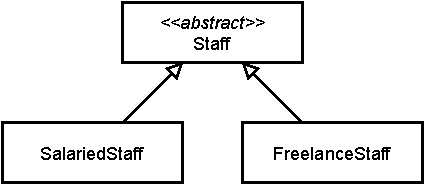
\includegraphics[height=.2\linewidth]{uml-inheritance}
    \caption{We hebben twee soorten staff: in vaste dienst of freelance.}
    \label{fig:uml-inheritance}
\end{figure}

Van \texttt{Staff} kunnen we een abstract class maken 
om bepaald gedrag te hergebruiken dat kenmerkend is voor personeel, zonder 
dat Staff op zichzelf geïnstantieerd kan worden. 
In de subklassen kunnen we dan overschrijven
wat specifiek verschilt in die klassen. Hierbij kan je bijvoorbeeld denken aan 
hoeveel er voor iemand betaald moet worden in loondienst versus als freelancer 
en hoeveel er afgedragen moet worden aan belastingen en sociale zekerheid.

\subsubsection{Realisatie (`implementeert')}
Realisatie of implementatie (\textit{interface inheritance}) geeft ook aan 
dat een subklasse een specifieke soort is van de interface, maar het is 
niet de bedoeling om zaken te overerven van het supertype. De insteek van 
een interface is om uitwisselbaarheid van implementaties te vergroten zonder 
de invulling van parent en child aan elkaar te koppelen.

\blockquote{
    A realization is a semantic relationship between classifiers
    in which one classifier specifies a contract that another
    classifier guarantees to carry out. 
}{\cite{Booch1999}, p. 149.}

Een typisch voorbeeld is de implementatie van een gateway: 
een toegangspoortje naar buiten toe, waarbij de onderliggende 
techniek kan worden uitgewisseld. Denk bijvoorbeeld aan het opslaan 
van cursussen in ons onderwijssysteem. Het feit dat we willen opslaan en uitlezen 
nemen we op in de interface. Hóe dat precies gebeurt vinden we in een implementatie.
In Figuur~\ref{fig:uml-realisation} zien we dit weergegeven: we kunnen ervoor 
kiezen om cursussen op te slaan in het bestandssysteem of in een database.

\begin{figure}[H]
    \centering
    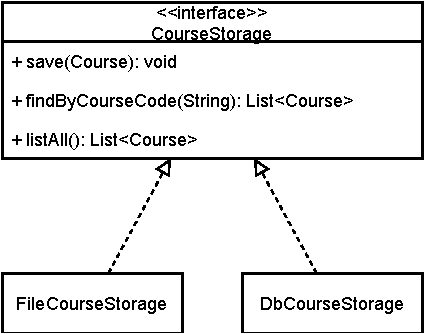
\includegraphics[height=.4\linewidth]{uml-realisation}
    \caption{De interface schrijft voor wat een CourseStorage allemaal moet kunnen. De implementaties moeten daaraan voldoende.}
    \label{fig:uml-realisation}
\end{figure}

Beide klassen zullen de methodes bevatten die worden afgedwongen door de 
interface.

\subsubsection{Subtyping, polymorfisme en dynamic binding}
De werkende principes achter overerving en realisatie zijn te vinden in 
subtyping, polymorfisme en dynamic binding.

\textit{Subtyping} houdt in dat het mogelijk is om een type-hiërarchie te hebben.
In Java is elk object bijvoorbeeld van het type Object, maar zitten er specifiekere
types onder. We kunnen subtypes definiëren door een klasse te extenden of 
een interface te implementeren. In Java kunnen klassen meerdere interfaces implementeren, 
maar slechts 1 klasse tegelijkertijd overerven. Het is wel mogelijk om het subtype verder 
steeds te extenden. Bij het verwijzen naar het type van een subklasse kan je altijd 
verwijzen naar het supertype (de interface of superklasse). Andersom is niet mogelijk.

\textit{Polymorfisme} (\textit{polymorphism}) is uit te leggen 
aan de hand van het woord zelf. Enerzijds herkennen we
het voorvoegsel \textit{poly-} (van het Griekse `πολύς', dat \textit{veel} of betekent), 
anderzijds herkennen we het woord \textit{-morfisme} (van `μορφή', dat \textit{vorm} betekent).
Polymorfisme kan men zien als `veelvormigheid': één abstractie kan verschillende vormen aannemen.
Anders gezegd: één supertype kan verschillende subtypen hebben.
Dit heeft als gevolg dat een methode, gespecificeerd in het supertype, 
in het subtype een andere vorm kan hebben. Het kan immers zijn geïmplementeerd of 
zijn overschreven.

\textit{Dynamic binding} is het mechanisme dat het in Java mogelijk maakt
een scheiding te hebben tussen de statische wereld van klassen tijdens compile time 
en de dynamische wereld van objecten tijdens runtime. Het houdt in dat
object-instanties van klassen \textit{tijdens runtime} met elkaar uitgewisseld 
worden als zij hetzelfde supertype hebben.

\blockquote{
Dynamic binding means that issuing a request doesn't commit you to a particular
implementation until run-time. Consequently, you can write programs that expect an
object with a particular interface, knowing that any object that has the correct interface
will accept the request. Moreover, dynamic binding lets you substitute objects that
have identical interfaces for each other at run-time. This substitutability is known as
\textbf{polymorphism}, and it's a key concept in object-oriented systems. It lets a client object
make few assumptions about other objects beyond supporting a particular interface.
Polymorphism simplifies the definitions of clients, decouples objects from each other,
and lets them vary their relationships to each other at run-time.
}{\cite{Gof1994}}

Subtyping, polymorfisme en dynamic binding zijn dan de sleutels 
tot flexibele object-georiënteerde software: het maakt het gemakkelijk 
om een afbakening aan te geven via interfaces of abstracte klassen 
waarvan de invulling later kan gebeuren of later vervangen kan worden.
De ene interface-implementatie kan uitgewisseld worden voor de andere,
zonder dat dat de rest van het systeem hoeft te verstoren!

\cite{Abelson1996}, paragraaf 2.4.2, noemen dit ook wel \textit{the principle of least commitment}:
subtyping, polymorfisme en dynamic binding geven ons de mogelijkheid om te koppelen tegen een (abstracte)
interface. Op die manier hoeven we ons nog niet vast te pinnen op een bepaalde implementatiekeuze!

\section{Samenvatting}
In dit hoofdstuk hebben we het object-georiënteerd modelleren en ontwerpen 
behandeld aan de hand van de belangrijkste onderdelen van het objectmodel van Booch.

\begin{defbox}{Belangrijkste elementen van het objectmodel van Booch}
    Het objectmodel van Booch onderscheid een aantal zaken
    die ons helpen goed gestructureerde object-georiënteerde software te ontwerpen:
    \begin{enumerate}
        \item \textbf{Abstraction}: klassen en objecten zijn onze kernabstracties waarin we 
        toestand (fields) en gedrag (methods) samenbrengen die bij elkaar horen. Dit verhoogt \textit{cohesion}.
        We kunnen met deze abstracties 
        communiceren via de publieke methoden. De interne werking hoeven we niet te weten (\textit{implementation hiding}).
        \item \textbf{Encapsulation}: hoe een abstractie zijn toestand bijhoudt en zijn 
        gedrag uitvoert wordt afgeschermd van de buitenwereld. Om \textit{information hiding} te bereiken wordt 
        gebruik gemaakt van access modifiers. Dit beperkt \textit{coupling}. Handige vuistregels om hierbij te helpen 
        zijn \textit{Tell, don't ask} en \textit{the Law of Demeter}.
        \item \textbf{Modularity}: klassen zijn modules waarin we toestand en gedrag samenbrengen. Daarnaast kennen 
        we interfaces om bepaald gedrag af te dwingen en enums om mogelijke waarden op te sommen. 
        Packages kunnen we gebruiken om klassen en andere modules te ordenen.
        \item \textbf{Hierarchy}: we kunnen packages onderbrengen in een logische, overzichtelijke ordening. Dat is onderdeel 
        van een softwarearchitectuur. Ook klassen en objecten kunnen in een hiërarchie tot elkaar staan. Er zijn namelijk 
        verschillende afhankelijkheden die tussen klassen kan gelden: \textit{dependency}, \textit{association}, \textit{aggregation},
        \textit{composition}, \textit{inheritance} en \textit{realisation}. Wat betreft inheritance en realisation zorgen 
        \textit{subtyping}, \textit{polymorphism} en \textit{dynamic binding} ervoor dat we een flexibele, uitwisselbare 
        invulling kunnen hebben van bepaalde abstracties. Eén abstractie kan namelijk verschillende vormen aannemen tijdens runtime:
        een subtype kan een implementatie of overschrijving verzorgen van het supertype.
    \end{enumerate}
\end{defbox}